\chapter{Cơ sở lý thuyết}
\section{Thư viện và công nghệ sử dụng}
\subsection{API}

Phần API trong hệ thống đóng vai trò là tầng trung gian giữa cơ sở dữ liệu và giao diện người dùng, thực hiện xử lý logic nghiệp vụ và cung cấp dữ liệu thông qua các endpoint RESTful. Việc thiết kế API dựa trên mô hình client-server giúp tách biệt phần backend và frontend, cho phép phát triển độc lập, mở rộng dễ dàng, và tăng tính bảo trì cho hệ thống. Dưới đây là các công nghệ và thư viện chính đã được sử dụng trong việc xây dựng API:

\begin{itemize}

    \item \textbf{Django}: 
    Django là một framework phát triển web mã nguồn mở được viết bằng ngôn ngữ Python, tuân theo triết lý ``Don't Repeat Yourself (DRY)'' và mô hình kiến trúc \textit{Model-View-Template (MVT)}. Django được thiết kế để giúp các lập trình viên phát triển ứng dụng nhanh chóng và an toàn. Một số tính năng nổi bật của Django bao gồm:
    \begin{itemize}
        \item \textit{ORM (Object-Relational Mapping)}: Cho phép ánh xạ các lớp Python thành bảng trong cơ sở dữ liệu quan hệ, giúp thao tác với dữ liệu bằng Python thay vì SQL thuần.
        \item \textit{Hệ thống authentication và authorization}: Django tích hợp sẵn mô hình người dùng, hệ thống phân quyền, bảo vệ dữ liệu người dùng.
        \item \textit{Hệ thống middleware}: Hỗ trợ xử lý các yêu cầu và phản hồi HTTP, tích hợp xác thực, logging, và các chức năng bảo mật như CSRF protection.
        \item \textit{Quản lý routing bằng URLconf}: Cho phép định tuyến URL tới các view tương ứng một cách rõ ràng và linh hoạt.
        \item \textit{Admin interface mạnh mẽ}: Giao diện quản trị tự động sinh từ các mô hình dữ liệu, giúp quản lý nội dung dễ dàng.
    \end{itemize}

    \item \textbf{Django REST Framework (DRF)}:
    Là một thư viện mở rộng mạnh mẽ của Django giúp xây dựng các API RESTful một cách hiệu quả. DRF trừu tượng hóa các thao tác với dữ liệu thông qua các lớp như \textit{Serializers}, \textit{Views}, và \textit{ViewSets}. Những tính năng nổi bật của DRF bao gồm:
    \begin{itemize}
        \item \textit{Serializers}: Chuyển đổi dữ liệu giữa dạng đối tượng Python và JSON/XML khi trao đổi qua HTTP.
        \item \textit{Generic Views / ViewSets / Routers}: Hỗ trợ định nghĩa các endpoint CRUD nhanh chóng chỉ với vài dòng code.
        \item \textit{Hệ thống xác thực}: Tích hợp sẵn các phương thức xác thực như Token, JWT, OAuth2, Session.
        \item \textit{Giao diện web test API}: Giao diện trực quan giúp kiểm thử và quan sát dữ liệu trả về từ endpoint dễ dàng.
        \item \textit{Pagination, Filtering, Throttling}: Hỗ trợ phân trang, lọc dữ liệu và giới hạn tốc độ truy cập để nâng cao hiệu suất.
    \end{itemize}

    \item \textbf{MongoEngine}:
    Là thư viện \textit{Object-Document Mapper (ODM)} dành cho MongoDB. Thay vì làm việc với tài liệu BSON trực tiếp, MongoEngine cho phép định nghĩa các mô hình Python tương tự Django ORM, giúp thao tác với MongoDB dễ dàng và trực quan hơn. Các đặc điểm chính:
    \begin{itemize}
        \item Cho phép ánh xạ cấu trúc tài liệu MongoDB vào các lớp Python.
        \item Hỗ trợ quan hệ giữa các tài liệu bằng kỹ thuật Reference và Embedded Document.
        \item Tương thích tốt với Django khi cấu hình chính xác.
    \end{itemize}

    \item \textbf{Django CORS Headers}:
    Đây là thư viện mở rộng giúp xử lý chính sách \textit{Cross-Origin Resource Sharing (CORS)} trong Django. Trong một hệ thống có frontend và backend tách rời (ví dụ: Angular ở cổng 4200, Django ở cổng 8000), trình duyệt sẽ chặn các yêu cầu không cùng nguồn (cross-origin) nếu không được cho phép. Django CORS Headers giúp cấu hình các domain nào được phép truy cập API Django, từ đó tránh lỗi CORS Policy.
    
    \item \textbf{Daphne}:
    Daphne là một máy chủ ứng dụng tương thích với chuẩn ASGI (Asynchronous Server Gateway Interface), được thiết kế để thay thế WSGI trong các ứng dụng cần giao tiếp bất đồng bộ như WebSocket hoặc các luồng realtime. Daphne là thành phần chính trong bộ Channels Stack, cho phép ứng dụng Django xử lý đồng thời nhiều kết nối bất đồng bộ, thích hợp cho các ứng dụng chat, livestream,...

    \item \textbf{Channels}:
    Channels mở rộng lõi đồng bộ của Django để hỗ trợ các giao thức bất đồng bộ như WebSocket, HTTP/2 hoặc các tác vụ nền. Channels sử dụng các thành phần như:
    \begin{itemize}
        \item \textit{Consumers}: Đóng vai trò tương tự như Views nhưng cho WebSocket, có thể xử lý các sự kiện kết nối, nhận, gửi dữ liệu.
        \item \textit{Channel Layer}: Lớp truyền thông cho phép các tiến trình giao tiếp với nhau thông qua hàng đợi.
        \item \textit{Redis}: Thường được dùng làm backend cho Channel Layer để đồng bộ dữ liệu giữa các tiến trình.
    \end{itemize}
    Việc tích hợp Channels giúp API có thể giao tiếp realtime với client mà không cần tải lại trang, ví dụ như hiển thị tin nhắn, thông báo,...

    \item \textbf{PyMongo}:
    PyMongo là thư viện chính thức từ MongoDB, dùng để thao tác với cơ sở dữ liệu MongoDB thông qua Python. Không giống MongoEngine, PyMongo làm việc trực tiếp với các tài liệu BSON, cho hiệu năng cao hơn và kiểm soát chặt hơn trong các truy vấn nâng cao. Các tính năng của PyMongo bao gồm:
    \begin{itemize}
        \item Kết nối tới MongoDB server qua URI, xác thực, và cấu hình SSL.
        \item Hỗ trợ truy vấn nâng cao, aggregation pipelines, index và thao tác tập hợp dữ liệu.
        \item Là thư viện chuẩn dùng trong các tác vụ có hiệu năng yêu cầu cao, hoặc xử lý dữ liệu phức tạp.
    \end{itemize}

\end{itemize}


\subsection{Frontend}

Phần frontend của ứng dụng đóng vai trò xây dựng giao diện người dùng (User Interface - UI) và tương tác trực tiếp với người dùng cuối. Tầng này được phát triển bằng các công nghệ hiện đại, đảm bảo hiệu suất cao, dễ bảo trì, đồng thời mang lại trải nghiệm người dùng trực quan và thân thiện. Dưới đây là các công nghệ chính được sử dụng:

\begin{itemize}

    \item \textbf{Angular}:
    Angular là một framework mã nguồn mở do Google phát triển, sử dụng ngôn ngữ TypeScript để xây dựng các ứng dụng web đơn trang (Single Page Application - SPA). Angular sử dụng kiến trúc \textit{Component-Based}, giúp tách biệt từng phần giao diện thành các module nhỏ, dễ dàng tái sử dụng và kiểm thử. Các tính năng chính bao gồm:
    \begin{itemize}
        \item \textit{Data Binding}: Hỗ trợ liên kết dữ liệu hai chiều (two-way binding) giữa giao diện và logic.
        \item \textit{Dependency Injection}: Cho phép quản lý và tái sử dụng các dịch vụ, giảm sự phụ thuộc giữa các thành phần.
        \item \textit{Routing Module}: Hỗ trợ chuyển đổi giữa các trang trong SPA mà không cần tải lại trang.
        \item \textit{Forms (Template-driven và Reactive Forms)}: Cho phép xây dựng các biểu mẫu linh hoạt, có kiểm tra và xác thực dữ liệu.
    \end{itemize}
    Trong đồ án này, Angular được sử dụng để xây dựng các thành phần giao diện như quản lý bài hát, album, danh sách phát và tính năng phát nhạc trực tuyến.

    \item \textbf{Tailwind CSS}:
    Tailwind CSS là một CSS framework dạng \textit{utility-first}, cung cấp các lớp tiện ích sẵn có để xây dựng giao diện mà không cần viết CSS thuần. Việc sử dụng Tailwind giúp:
    \begin{itemize}
        \item Tăng tốc quá trình thiết kế giao diện nhờ các lớp tiện ích sẵn.
        \item Đảm bảo giao diện đồng nhất, hiện đại và dễ tùy biến.
        \item Loại bỏ tình trạng CSS trùng lặp nhờ cơ chế tree-shaking tích hợp với build tool như Vite hoặc Webpack.
    \end{itemize}
    Trong ứng dụng, Tailwind CSS được sử dụng để thiết kế các thành phần như bảng dữ liệu, nút điều khiển, layout chính, form nhập liệu và phần phát nhạc.

    \item \textbf{RxJS (Reactive Extensions for JavaScript)}:
    RxJS là một thư viện lập trình phản ứng (reactive programming) dựa trên luồng dữ liệu bất đồng bộ (asynchronous data streams). Angular tích hợp sâu với RxJS thông qua \texttt{Observable}, giúp:
    \begin{itemize}
        \item Quản lý dữ liệu từ API một cách linh hoạt.
        \item Đồng bộ hóa trạng thái ứng dụng theo thời gian thực.
        \item Xử lý các thao tác bất đồng bộ như HTTP request, WebSocket, sự kiện DOM.
    \end{itemize}
    Việc sử dụng RxJS giúp frontend hoạt động hiệu quả trong việc cập nhật dữ liệu liên tục mà không gây tải lại trang.

    \item \textbf{TypeScript}:
    TypeScript là một siêu ngôn ngữ của JavaScript, bổ sung hệ thống kiểu tĩnh (static typing) cùng với các tính năng hướng đối tượng mạnh mẽ. Những ưu điểm của TypeScript bao gồm:
    \begin{itemize}
        \item Dễ phát hiện lỗi tại thời điểm biên dịch (compile-time).
        \item Hỗ trợ kiểm tra và gợi ý thông minh từ trình soạn thảo (IntelliSense).
        \item Dễ bảo trì và mở rộng hệ thống nhờ tính rõ ràng của mã nguồn.
    \end{itemize}
    Trong đồ án, toàn bộ mã nguồn frontend được phát triển bằng TypeScript để đảm bảo độ ổn định, khả năng kiểm soát logic ứng dụng và dễ dàng bảo trì trong các giai đoạn nâng cấp sau này.

\end{itemize}


\section{Cấu trúc mã nguồn}
\subsection{API}
Cấu trúc thư mục chính của phần API được tổ chức như sau:
\begin{itemize}
    \item \textbf{spotify-api/}: Thư mục chính chứa mã nguồn API.
    \begin{itemize}
        \item \textbf{settings.py}: File cấu hình chính của Django, chứa các thông tin như cấu hình cơ sở dữ liệu, ứng dụng cài đặt, và các thông số bảo mật.
        \item \textbf{urls.py}: File định tuyến URL, ánh xạ các endpoint API đến các view tương ứng.
        \item \textbf{models.py}: File định nghĩa các mô hình dữ liệu, bao gồm các bảng và quan hệ trong cơ sở dữ liệu.
        \item \textbf{views.py}: File xử lý logic cho các endpoint API, bao gồm các chức năng như đăng ký, đăng nhập, và quản lý người dùng.
        \item \textbf{serializers.py}: File chuyển đổi dữ liệu giữa mô hình Python và định dạng JSON để giao tiếp với frontend.
    \end{itemize}
    \item \textbf{requirements.txt}: File liệt kê các thư viện cần thiết để chạy API, giúp dễ dàng cài đặt môi trường phát triển.
\end{itemize}

\subsection{Frontend}
Cấu trúc thư mục chính của phần frontend được tổ chức như sau:
\begin{itemize}
    \item \textbf{src/}: Thư mục chính chứa mã nguồn Angular.
    \begin{itemize}
        \item \textbf{app/}: Chứa các component và service chính
        \begin{itemize}
            \item \textbf{admin/}: Chứa các component quản trị như \texttt{admin-dashboard-management}, \texttt{admin-user-management}, \texttt{admin-album-management}, \texttt{admin-songs-management}, \texttt{admin-artist-management}.
            \item \textbf{shared/}: Chứa các component dùng chung như \texttt{toast-message}.
            \item \textbf{services/}: Chứa các service như \texttt{login.service.ts}, \texttt{songs.service.ts}, \texttt{artists.service.ts}.
            \item \textbf{components khác}: Các component chính như \texttt{profile}, \texttt{my-play-list}, \texttt{album}, \texttt{detail}, \texttt{login}, \texttt{register}, \texttt{video}.
        \end{itemize}
        \item \textbf{assets/}: Chứa các tài nguyên như hình ảnh (\texttt{Img/}), file CSS, và các tài nguyên tĩnh khác.
        \item \textbf{environments/}: Chứa cấu hình môi trường (\texttt{environment.ts} cho dev, \texttt{environment.prod.ts} cho production).
    \end{itemize}
    \item \textbf{angular.json}: File cấu hình dự án Angular, định nghĩa các thông số build, serve, và cấu trúc dự án.
    \item \textbf{package.json}: Danh sách các thư viện cần thiết cho frontend, bao gồm các dependency như \texttt{@angular/core}, \texttt{rxjs}, \texttt{tailwindcss}.
    \item \textbf{tailwind.config.js}: File cấu hình Tailwind CSS, định nghĩa các lớp utility được sử dụng trong dự án.
\end{itemize}

\section{Mô hình ứng dụng và các tính năng}
\subsection{Mô hình tổng thể}
Hệ thống được xây dựng theo mô hình \textbf{client-server}, trong đó hai thành phần chính là \textbf{Backend API} và \textbf{Frontend} phối hợp chặt chẽ để cung cấp các chức năng của ứng dụng. 

\textbf{Phần Backend API} chịu trách nhiệm xử lý toàn bộ logic nghiệp vụ, xác thực người dùng, và quản lý dữ liệu. API được xây dựng trên nền tảng \textbf{Django REST Framework (DRF)}, sử dụng cơ sở dữ liệu \textbf{MongoDB} để lưu trữ thông tin như người dùng, bài hát, danh sách phát, và các dữ liệu liên quan. Backend API cung cấp các endpoint RESTful để frontend có thể giao tiếp, đảm bảo tính bảo mật và hiệu suất cao.

\textbf{Phần Frontend} được phát triển bằng \textbf{Angular}, cung cấp giao diện người dùng hiện đại, thân thiện và dễ sử dụng. Frontend chịu trách nhiệm hiển thị dữ liệu từ API, đồng thời cho phép người dùng thực hiện các thao tác như đăng ký, đăng nhập, tìm kiếm bài hát, quản lý danh sách phát, và phát nhạc trực tuyến. Giao tiếp giữa frontend và backend được thực hiện thông qua các yêu cầu HTTP với dữ liệu được trao đổi dưới định dạng JSON.

Mô hình này đảm bảo tính phân tách rõ ràng giữa giao diện người dùng và logic xử lý phía server, giúp hệ thống dễ dàng mở rộng, bảo trì và tích hợp thêm các tính năng mới trong tương lai.

\subsection{Các tính năng được xây dựng}
Hệ thống được thiết kế và phát triển với các tính năng chính, bao gồm cả phần \textbf{API} và \textbf{Frontend}, nhằm đáp ứng nhu cầu quản lý và phát nhạc trực tuyến.

\begin{itemize}
    \item \textbf{Đăng ký và đăng nhập người dùng}:
    \begin{itemize}
        \item Cho phép người dùng tạo tài khoản mới và đăng nhập vào hệ thống.
        \item Hỗ trợ xác thực thông qua email và mật khẩu.
    \end{itemize}
    \item \textbf{Xác thực và phân quyền người dùng}:
    \begin{itemize}
        \item Sử dụng token để xác thực người dùng, đảm bảo chỉ những người dùng hợp lệ mới có thể truy cập các tài nguyên.
        \item Phân quyền người dùng dựa trên vai trò (admin, user) để kiểm soát quyền truy cập vào các chức năng cụ thể.
    \end{itemize}
    \item \textbf{Quản lý thông tin người dùng (CRUD)}:
    \begin{itemize}
        \item Cho phép thêm, sửa, xóa và xem thông tin người dùng.
        \item Hỗ trợ quản trị viên quản lý danh sách người dùng trong hệ thống.
    \end{itemize}
    \item \textbf{Quản lý nội dung âm nhạc}:
    \begin{itemize}
        \item Quản lý danh sách bài hát, bao gồm các chức năng thêm, sửa, xóa và tìm kiếm bài hát.
        \item Quản lý album nhạc, cho phép người dùng tạo và chỉnh sửa album cá nhân.
        \item Quản lý danh sách phát nhạc của người dùng.
    \end{itemize}
    \item \textbf{Phát nhạc và video âm nhạc}:
    \begin{itemize}
        \item Cung cấp URL phát nhạc và video trực tuyến, hỗ trợ các định dạng phổ biến.
    \end{itemize}
\end{itemize}


\subsection{Flowchart hoạt động}
\begin{figure}[h]
    \centering
    % \includegraphics[width=0.8\textwidth]{imgs/system-flowchart.png}
    \caption{Flowchart hoạt động của hệ thống}
\end{figure}

\section{Thiết kế cơ sở dữ liệu}
Cơ sở dữ liệu của dự án sử dụng MongoDB, một hệ quản trị cơ sở dữ liệu NoSQL, để lưu trữ và quản lý dữ liệu. Các bảng chính trong cơ sở dữ liệu bao gồm:

\begin{itemize}
    \item \textbf{User}: Lưu trữ thông tin người dùng, bao gồm:
    \begin{itemize}
        \item \textbf{email}: Địa chỉ email của người dùng.
        \item \textbf{password}: Mật khẩu đã được mã hóa.
        \item \textbf{username}: Tên đăng nhập của người dùng.
        \item \textbf{is\_staff}: Trạng thái nhân viên (true/false).
        \item \textbf{is\_superuser}: Trạng thái quản trị viên (true/false).
    \end{itemize}

    \item \textbf{Playlist}: Lưu trữ danh sách phát nhạc của người dùng, bao gồm:
    \begin{itemize}
        \item \textbf{title}: Tên danh sách phát.
        \item \textbf{user}: ID của người dùng sở hữu danh sách phát.
        \item \textbf{songs}: Danh sách các bài hát trong danh sách phát (danh sách các ID bài hát).
    \end{itemize}

    \item \textbf{Song}: Lưu trữ thông tin bài hát, bao gồm:
    \begin{itemize}
        \item \textbf{title}: Tên bài hát.
        \item \textbf{artist}: Danh sách các nghệ sĩ liên quan đến bài hát.
        \item \textbf{file\_location}: Đường dẫn phát nhạc (URL đến file nhạc trên S3).
        \item \textbf{image\_location}: Đường dẫn hình ảnh đại diện của bài hát.
        \item \textbf{genre}: Thể loại nhạc.
        \item \textbf{duration}: Thời lượng bài hát.
        \item \textbf{lyrics}: Lời bài hát.
    \end{itemize}

    \item \textbf{Album}: Lưu trữ thông tin album nhạc, bao gồm:
    \begin{itemize}
        \item \textbf{title}: Tên album.
        \item \textbf{release\_date}: Ngày phát hành album.
        \item \textbf{album\_type}: Loại album (ví dụ: single, album đầy đủ).
        \item \textbf{artist\_ids}: Danh sách các ID nghệ sĩ liên quan đến album.
        \item \textbf{song\_ids}: Danh sách các ID bài hát trong album.
        \item \textbf{album\_photo}: Đường dẫn hình ảnh đại diện của album.
    \end{itemize}

    \item \textbf{Artist}: Lưu trữ thông tin nghệ sĩ, bao gồm:
    \begin{itemize}
        \item \textbf{name}: Tên nghệ sĩ.
        \item \textbf{bio}: Tiểu sử của nghệ sĩ.
        \item \textbf{debut\_year}: Năm ra mắt.
        \item \textbf{artist\_photo}: Đường dẫn hình ảnh đại diện của nghệ sĩ.
    \end{itemize}
\end{itemize}

\subsection{Mối quan hệ giữa các bảng}
\begin{itemize}
    \item \textbf{User} có thể sở hữu nhiều \textbf{Playlist}.
    \item \textbf{Playlist} chứa nhiều \textbf{Song}.
    \item \textbf{Album} chứa nhiều \textbf{Song} và liên kết với nhiều \textbf{Artist}.
    \item \textbf{Song} có thể liên kết với nhiều \textbf{Artist}.
\end{itemize}

\subsection{Sơ đồ ERD}
\begin{figure}[h]
    \centering
    % 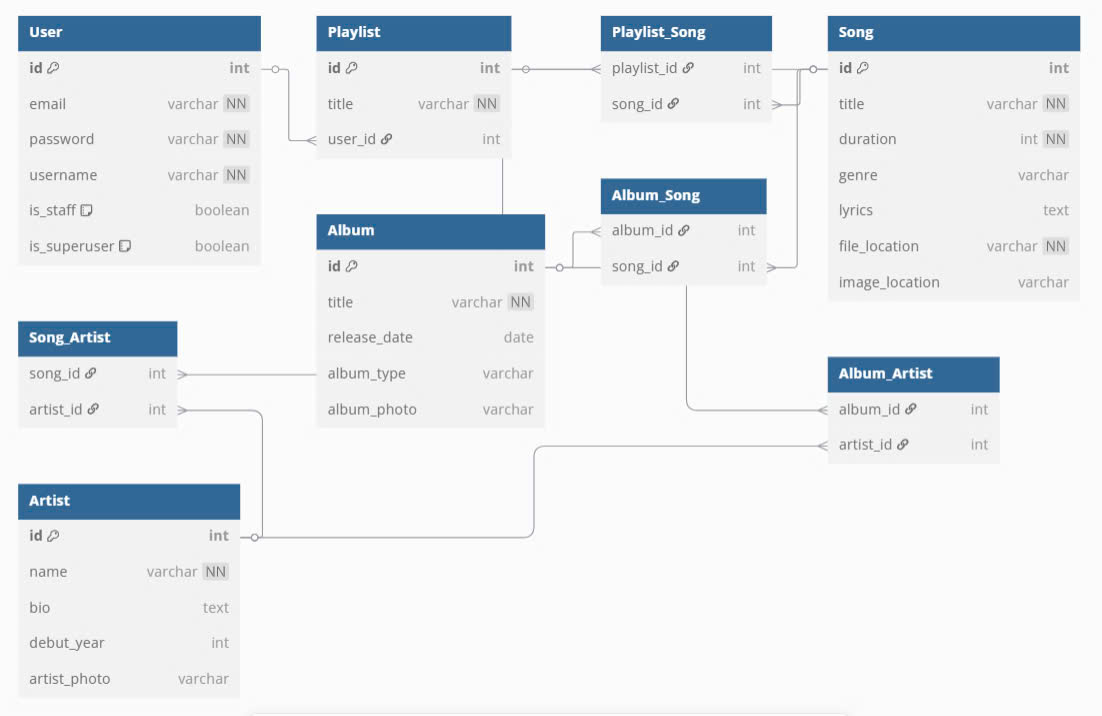
\includegraphics[width=0.8\textwidth]{imgs/erd.png}
    \caption{Sơ đồ ERD của cơ sở dữ liệu}
\end{figure}
